%----------------------------------------------------------------------------------------
%	TITLE PAGE
%----------------------------------------------------------------------------------------
%%%%%%%%%%%%%%%%%%%%%%%%%%%%%%%%%%%%%%%%%
% Beamer Presentation
% LaTeX Template
% Version 1.0 (10/11/12)
%
% This template has been downloaded from:
% http://www.LaTeXTemplates.com
%
% License:
% CC BY-NC-SA 3.0 (http://creativecommons.org/licenses/by-nc-sa/3.0/)
%
%%%%%%%%%%%%%%%%%%%%%%%%%%%%%%%%%%%%%%%%%

%----------------------------------------------------------------------------------------
%	PACKAGES AND THEMES
%----------------------------------------------------------------------------------------

\documentclass{beamer}

\mode<presentation> {

% The Beamer class comes with a number of default slide themes
% which change the colors and layouts of slides. Below this is a list
% of all the themes, uncomment each in turn to see what they look like.

% \usetheme{default}
%\usetheme{AnnArbor}
%\usetheme{Antibes}
%\usetheme{Bergen}
%\usetheme{Berkeley}
%\usetheme{Berlin}
%\usetheme{Boadilla}
%\usetheme{CambridgeUS}
%\usetheme{Copenhagen}
% \usetheme{Darmstadt}
%\usetheme{Dresden}
%\usetheme{Frankfurt}
%\usetheme{Goettingen}
%\usetheme{Hannover}
%\usetheme{Ilmenau}
%\usetheme{JuanLesPins}
%\usetheme{Luebeck}
\usetheme{Madrid}
%\usetheme{Malmoe}
%\usetheme{Marburg}
% \usetheme{Montpellier}
%\usetheme{PaloAlto}
%\usetheme{Pittsburgh}
%\usetheme{Rochester}
%\usetheme{Singapore}
%\usetheme{Szeged}
%\usetheme{Warsaw}

% As well as themes, the Beamer class has a number of color themes
% for any slide theme. Uncomment each of these in turn to see how it
% changes the colors of your current slide theme.

%\usecolortheme{albatross}
%\usecolortheme{beaver}
%\usecolortheme{beetle}
%\usecolortheme{crane}
%\usecolortheme{dolphin}
%\usecolortheme{dove}
%\usecolortheme{fly}
%\usecolortheme{lily}
%\usecolortheme{orchid}
%\usecolortheme{rose}
% \usecolortheme{seagull}
% \usecolortheme{seahorse}
\usecolortheme{whale}
%\usecolortheme{wolverine}

%\setbeamertemplate{footline} % To remove the footer line in all slides uncomment this line
%\setbeamertemplate{footline}[page number] % To replace the footer line in all slides with a simple slide count uncomment this line

\setbeamertemplate{navigation symbols}{} % To remove the navigation symbols from the bottom of all slides uncomment this line
}

%----------------------------------------------------------------------------------------
%	PACKAGES
%----------------------------------------------------------------------------------------

\usepackage{booktabs} % Allows the use of \toprule, \midrule and \bottomrule in tables
% ------- Français -----------	
\usepackage[francais]{babel}
\usepackage[utf8]{inputenc}
\usepackage[T1]{fontenc}
%
\usepackage{graphicx}
% \usepackage{subfigure}
% \usepackage{float}
% \usepackage{lmodern}
% \usepackage{ae,aecompl}
% \usepackage{enumitem}
% \usepackage{scalerel}
% \usepackage{textcomp}
% % --------------------------------	
% %	Caractères mathématiques
% \usepackage{amsmath}
% \usepackage{systeme}
% \usepackage{amsfonts}
% \usepackage{mathabx}
%
% % Vector column type
% \newcount\colveccount
% \newcommand*\colvec[1]{
%         \global\colveccount#1
%         \begin{pmatrix}
%         \colvecnext
% }
% \def\colvecnext#1{
%         #1
%         \global\advance\colveccount-1
%         \ifnum\colveccount>0
%                 \\
%                 \expandafter\colvecnext
%         \else
%                 \end{pmatrix}
%         \fi
% }
%    

% ======================
% 		GRAPHIC
% \usepackage{amssymb}
% \usepackage{xcolor}


\title[]{APP Vents 1: Percer les mystères des perces de cuivres} % The short title appears at the bottom of every slide, the full title is only on the title page

\author{Groupe B} % Your name
\institute[ATIAM] % Your institution as it will appear on the bottom of every slide, may be shorthand to save space
{
Master ATIAM, Acoustique } % Your institution for the title page
\medskip
\date{\today} % Date, can be changed to a custom date

\begin{document}

\begin{frame}
\titlepage % Print the title page as the first slide
\end{frame}

\begin{frame}
  \frametitle{Hypothèses}
  \begin{enumerate}
    \item \textbf{Régime linéaire:} petites perturbations
    \item \textbf{Hypothèse basse fréquences:} $ka <<1$
    \item \textbf{Géométrie simple:} segments coniques ou cylindriques
    \item \textbf{Tuyau large:} $a >> r_v$
  \end{enumerate}
\end{frame}

% =========================

\begin{frame}
  \frametitle{Modèle conservatif VS dissipatif (1/2)}
\begin{block}{Impédance d'entrée d'un cylindre}
  Longueur $L$ fermé-ouvert
  \begin{equation*}
    Z_e = \mbox{j} \frac{\rho_0 c}{S} \tan{kL} =  \mbox{j} Z_c \tan{kL}
 \end{equation*}
 \end{block}


 \pause
 \begin{exampleblock}{Introduction des pertes}
 On considère les deux modèles suivants:
  \begin{itemize}
    \item \textbf{Conservatif:} $k = \frac{w}{c}$
    \item \textbf{Dissipatif:} $k_c = k + \alpha (1 - \mbox{j})$, \hspace{20pt}
    $\alpha = 3.10^{-5} \sqrt{\frac{f}{R}}$
  \end{itemize}
 \end{exampleblock}

  \pause
  \begin{block}{Modèle dissipatif}
    \begin{itemize}
      \item L'impédance dissipative comprend une \textbf{partie réelle résistive} 
        et une \textbf{partie imaginaire réactive} (correction de longueur).
      \pause
      \item Fréquences $f_n$ plus basses et amortissement des pics d'impédance
    \end{itemize}
  \end{block}
\end{frame}

% =========================

\begin{frame}
  \frametitle{Modèle conservatif VS dissipatif (2/2)}
    \begin{figure}
      \centering
      \captionsetup{justification=centering, margin=1cm}
      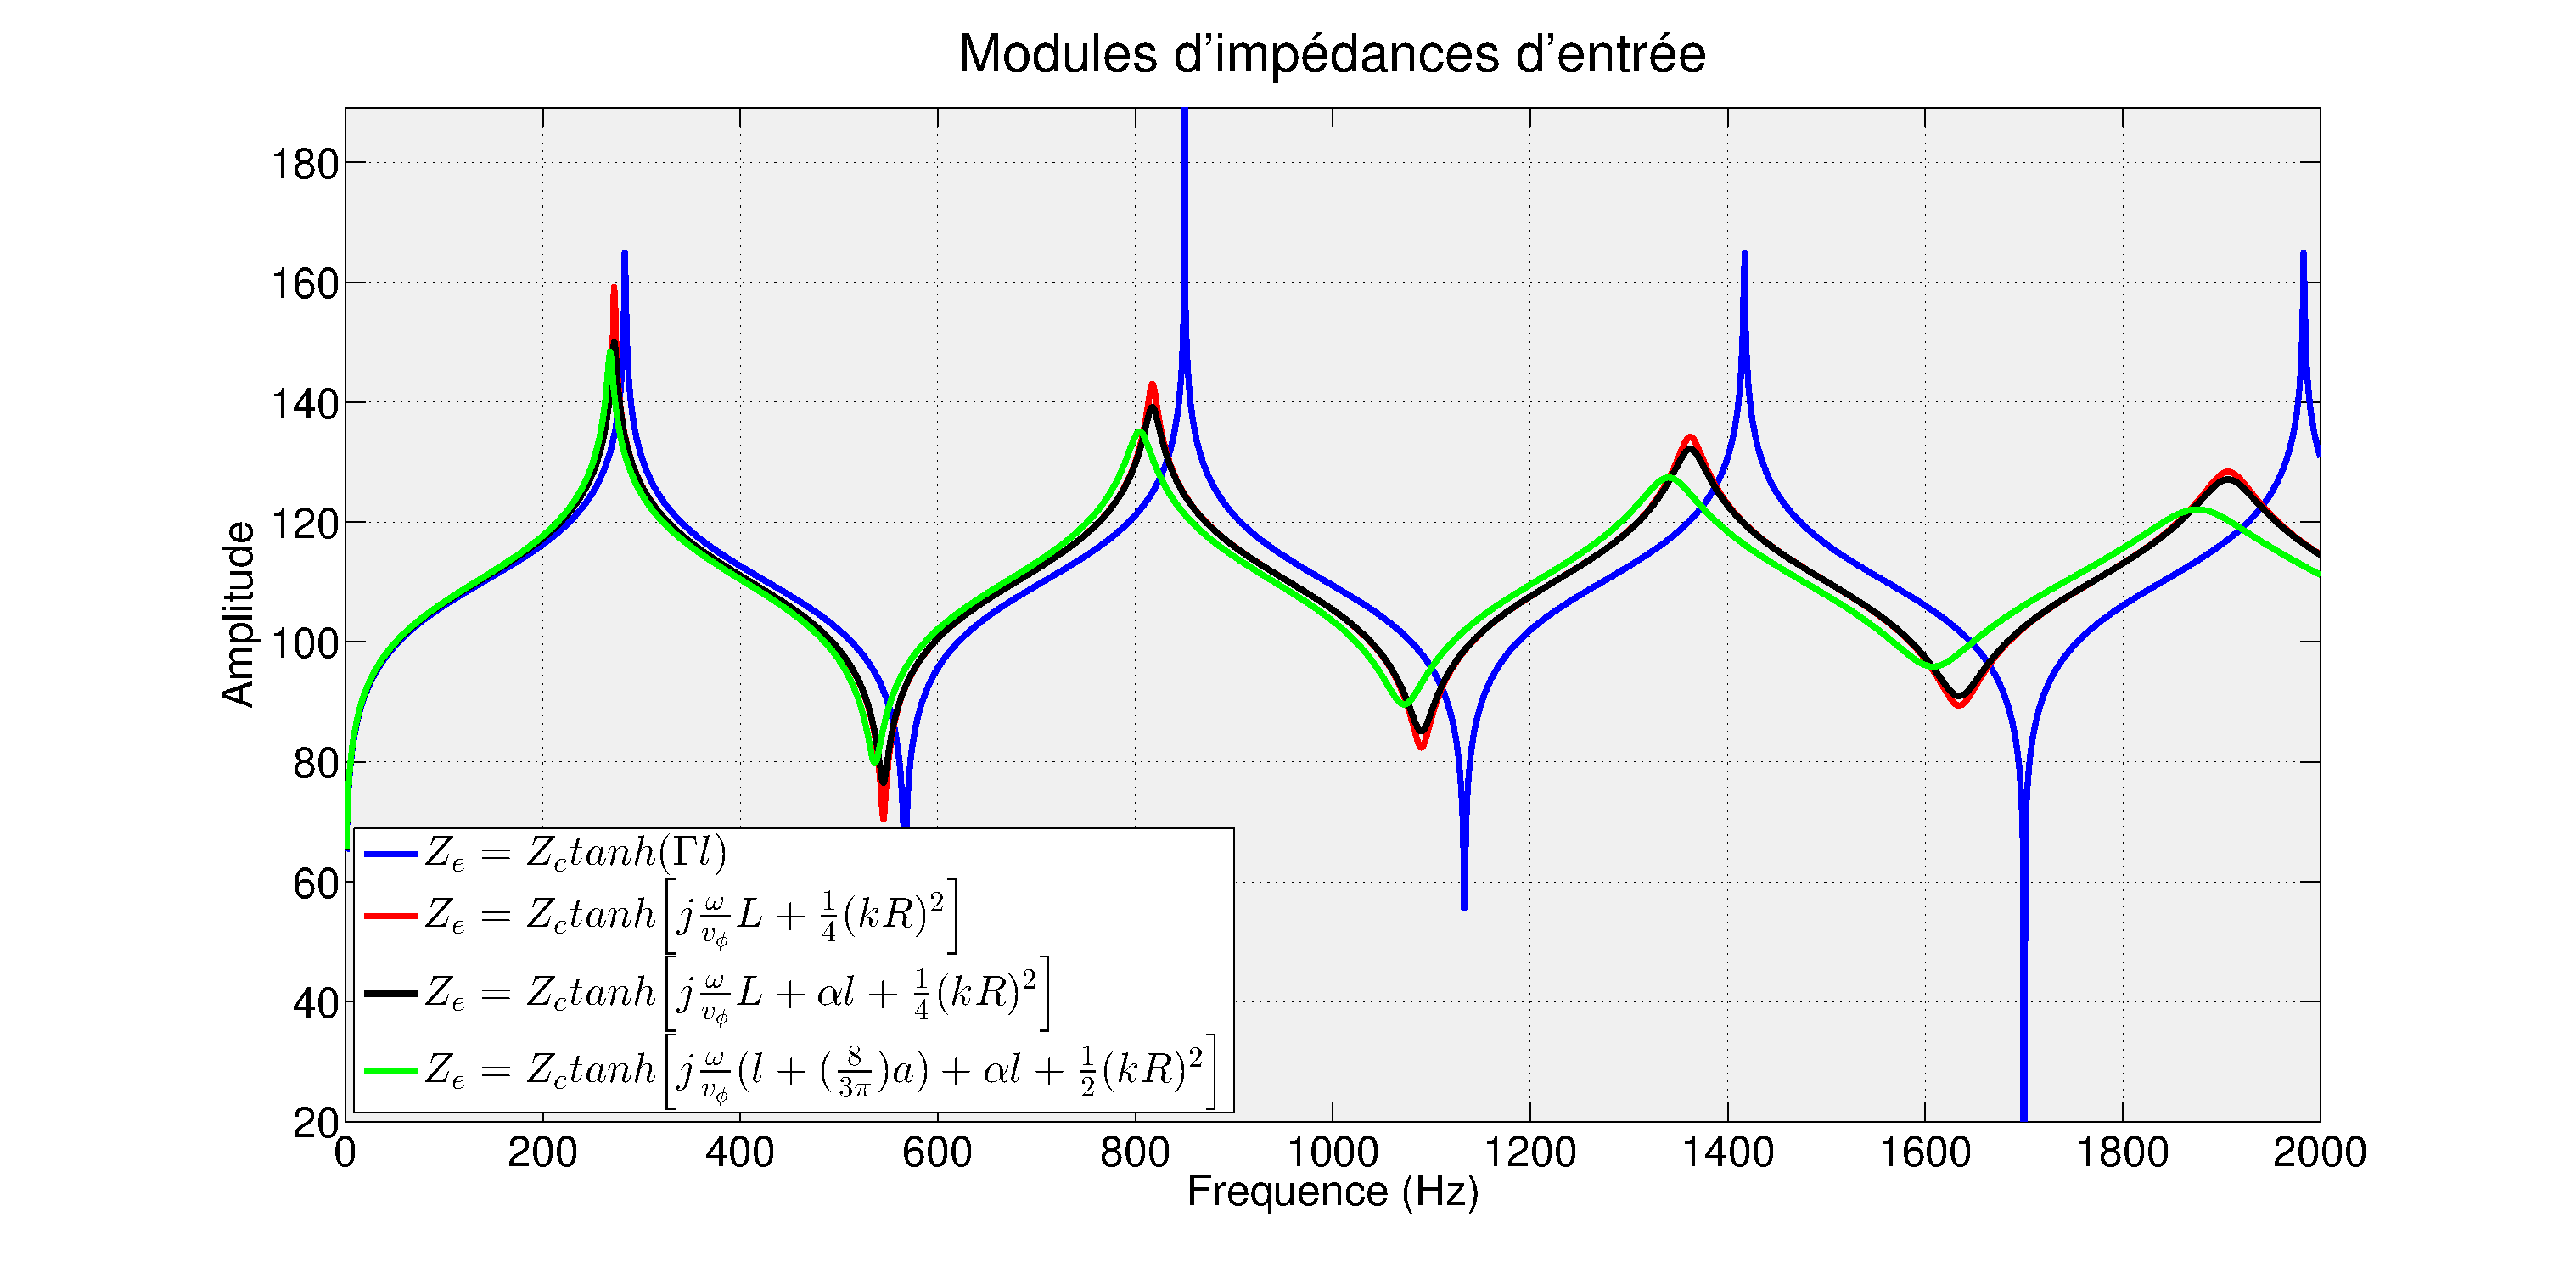
\includegraphics[width=0.85\textwidth]{img/imp_entree3.eps}
      \caption{Impédance d'entrée d'un cylindre;
              {\color{blue} En bleu}, modèle conservatif; 
               \alert{En rouge}, modèle dissipatif;
               {\textbf{En noir}, cas baflé},
               {\color{green}En vert}, cas non-baflé
              }
    \end{figure}
    \begin{center}
      \alert{Les maxima locaux de l'impédance sont les fréquences de résonance}
    \end{center}
\end{frame}

% =========================
\begin{frame}
  \frametitle{Prise en compte du rayonnement}
  \begin{exampleblock}{Modèle dissipatif}
    \begin{itemize}
    \item Correction de longueur de l'ordre de $0.6 R$
    \item écart en cent: $1200 \log_2 (\frac{f_2}{f_1}) = 68 $ (cas baflé)
    \item Dans le cas non-baflé: $c = 98 cents$
    \end{itemize}

    \end{exampleblock}
\pause
    \begin{block}{Rayonnement}
  \begin{itemize}
    \item L'impédance à l'extrémité ouverte n'est plus nulle.
    \item Pertes très petites
    \item On pose $Z(x = L) = Z_r$
  \end{itemize}
\end{block}
\end{frame}

% =========================

\begin{frame}
  \frametitle{Outil numérique d'estimation d'impédance d'entrée}
  
  \pause
  \begin{block}{Matrice de Transfert}
    Permet de donner d'obtenir l'impédance à une abscisse $x_1$ du système à
    partir de l'impédance à l'abscisse $x_2$:
    \begin{equation*}
      \begin{pmatrix}
        p_1\\
        u_1\\
      \end{pmatrix}
      =
      \begin{pmatrix}
        A &B\\
        C &D\\
      \end{pmatrix}
      \begin{pmatrix}
        p_2\\
        u_2\\
      \end{pmatrix}
    \end{equation*}
  \end{block}

  \vspace{20pt}
  \pause
  \begin{exampleblock}{Algorithme}
  \begin{itemize}
    \item Les coefficients de la matrice sont calculés dans le cas d'un segment
  conique, qui se simplifie dans le cas cylindrique (e.g. $R(x_1) = R(x_2)$).
  \pause
    \item En partant de la fin, on calcule la matrice de transfert de chaque
      segment jusqu'à obtenir la matrice de transfert du système complet
  \end{itemize}
\end{exampleblock}
\end{frame}

% ========================
\begin{frame}
  \frametitle{Cas d'étude}
    \begin{figure}
      \centering
      \captionsetup{justification=centering, margin=1cm}
      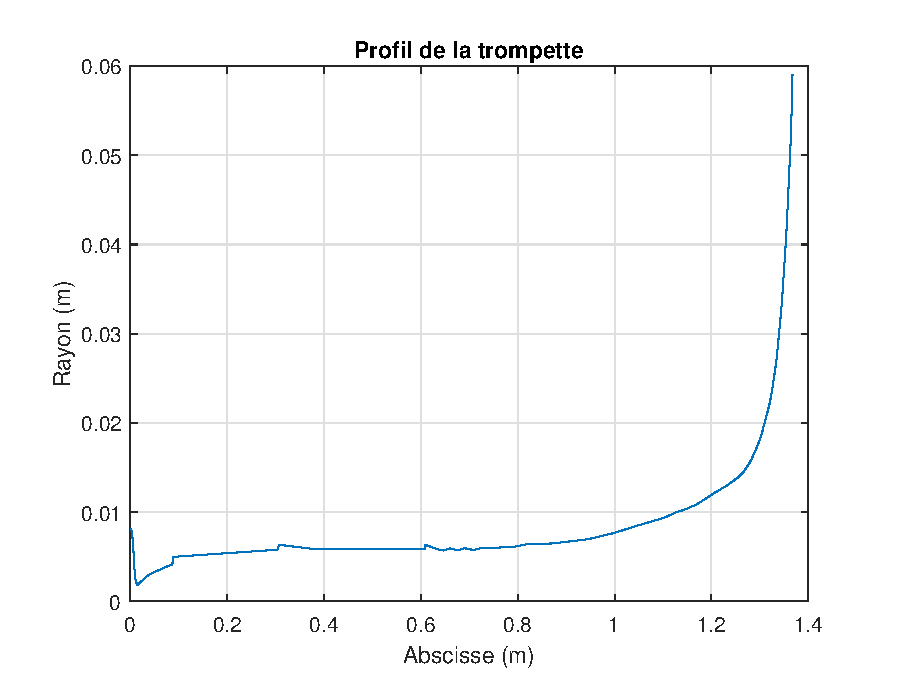
\includegraphics[width=0.7\textwidth]{img/prof_tromp.eps}
      \caption{Perce d'une trompette Bressing}
    \end{figure}
\end{frame}

\end{document}
